\documentclass{sig-alternate}
\usepackage{graphicx}
\usepackage{subfigure}
\usepackage{enumerate}
\usepackage{balance}  % for  \balance command ON LAST PAGE  (only there!)
%\usepackage{booktabs} % for better looking tables
\usepackage{wrapfig}
\usepackage{array}
\usepackage{multirow}

% For SQL and AWK code formatting:
\usepackage{listings}
\usepackage{color}
\definecolor{darkgray}{rgb}{0.6,0.6,0.6}
\definecolor{darkgreen}{rgb}{0.3,0.5,0.3}
\lstdefinestyle{SQL}{
  language=SQL,
  showstringspaces=false,
  basicstyle=\rm\ttfamily,
  backgroundcolor=\color{white},
  commentstyle=\ttfamily\itshape,
  keywordstyle=\ttfamily\color{darkgreen},
  morekeywords={FUNCTION, BOOLEAN, RETURNS, DETERMINISTIC, RETURN, REFERENCES, WITH, SEQUENCE, TRUNCATE, START, RULE, TO, DO, IS, INSTEAD, NEW, PARTITION, RANK},
  stringstyle=\ttfamily\color{blue},
  breaklines=true,
  framexleftmargin=0.5em,
  frame=single,
  rulecolor=\color{black},
  rulesepcolor=\color{darkgray},
  xleftmargin=1em,
  xrightmargin=1em,
  columns=fixed
}

\newcommand{\hide}[1]{}
\sloppy

\usepackage{PDBF}

\DBSQLFile{somedb.sql}
\DBSQLJDBC{jdbc:postgresql://localhost:5432/postgres}{postgres}{test}{testtest, dim_time, dim_compiler, dim_dataset, dim_implementation, dim_layout, dim_query, dim_machine, fact_experiment}
\renewcommand\pdbfScale{1.00}
\renewcommand\pdbfQuality{1.00}
  
\begin{document}

\title{The Surprising Runtime Fragility Found when Querying a Single Table}
\title{On the Surprising Runtime Fragility Found when Querying a Single Table}
\subtitle{\vspace*{-0.4cm}[Experiments and Analysis Mini-Paper]}

\numberofauthors{1} 

\author{
\alignauthor
Endre Palatinus \hspace{0.5cm} Jens Dittrich 
\\\vspace*{0.2cm}
\affaddr{Information Systems Group, Saarland University}\\
\affaddr{http://infosys.cs.uni-saarland.de}\\
}

\date{}

\maketitle

\section{Problem statement}

Given a table with two attributes and a simple query reading those attributes, which data layout (row, column or a suitable PAX-layout) should we choose in order to get the best possible performance? This sounds really simple, yet this paper shows it is not. We will explore the parameter space that has an impact on the performance of such queries including: (1)~the data type used in the schema, (2)~branches in the code, (3)~the CPU architecture, (4)~the compiler, (5)~the optimization level, as well as (6)~compile time vs. runtime layouts. In addition, we will show that a task like this is not easy to measure as we observe considerable variance throughout our measurements which makes it difficult to argue along means over different runs of an experiment. Therefore, we compute confidence intervals for all measurements and exploit this to detect outliers and define classes of methods that we are not allowed to distinguish statistically.
Our results indicate that a carefully or ill-chosen compilation setup can trigger a performance gain or loss of factor~1.6 to factor~28, depending on the setup. We also introduce robustness graphs displaying the impact of non-optimal layouts on runtime performance.
Finally, we give a clear guideline on when to use which method.

%TODO \vspace{-0.3cm}
\section{Data Layouts in Main Memory}
\label{sec:layouts}

The two most common data layouts used in todays database management systems are row and column layout. These are only the two extremes when vertically partitioning a table. In-between these extremes there exists a full spectrum of column-grouped layouts, which under certain settings can beat both of the aforementioned traditional layouts for legacy disk-based row-stores~\cite{VP}. However, for main-memory systems column grouped layouts have not proved to be of much use for OLTP workloads~\cite{grund2010hyrise}, unless the schema is very wide~\cite{JITHybrid}.

Another axis of partitioning a table is horizontal partitioning. This is usually based on the values of a column with low cardinality, e.g.~geographical regions, but this is not necessarily a requirement. Therefore an alternative to laying out all records of a table in column layout is to do this \textit{within} horizontal partitions, so-called chunks of the table. This can be done e.g.~by taking repeatedly $k$~records from the table and laying them out in column layout. We denote the special case when $k=2^N$ by \mbox{ColumnXN}. Row layout is the same as ColumnX0, and column layout is equivalent to ColumnXN, where $2^N$ is larger or equal to the cardinality of the table. The chunks of these layouts are analogous to PAX~pages~\cite{PAX}, however, we can choose any chunk size that is a multiple of the tuple size, while for PAX we are restricted to multiples of the disk's block size. The possible horizontal partitionings of a table having 2 columns and 8 records, using column layout inside the partitions are illustrated in Figure~\ref{fig:ColumnXN}. Here we can see the two extremes: row- and column layout, and chunked column layouts with a chunk-size of 2 (ColumnX1) and 4 (ColumnX2). 

\begin{figure}[!h]
\vspace{-5pt}
\center
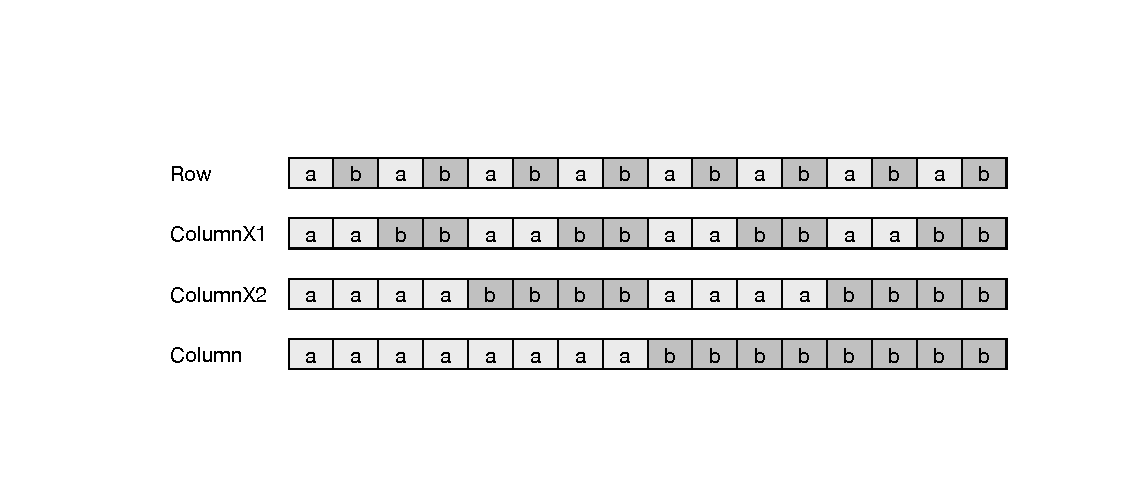
\includegraphics[width=0.45\textwidth]{pdf/ColumnXNIllustration.pdf}
\vspace{-10pt}
\caption{Horizontal partitionings of a table having 2 columns and 8 records, using column layout inside the partitions, and chunk sizes of powers of 2.}  
\label{fig:ColumnXN}
\vspace{-10pt}
\end{figure}


\section{The six-dimensional Parameter Space of our Experiments}

\noindent {\bf (1) The datatype used in the schema.} Our dataset is a single table with two integer columns, with a total size of 2~GB. Depending on the data type chosen (1-byte, 4-byte, or 8-byte integers) we get the following scenarios:

\begin{table}[!ht]
  \vspace{-5pt}
  \scriptsize
  \centering
  \begin{tabular}{| l | l | r |}
    \hline
    {\bf Label} & {\bf Schema} & {\bf Tuple count} \\ \hline \hline
    char & \texttt{Table\_char (a int1, b int1)} & 1024 * 1024 * 1024 \\ \hline
    int & \texttt{Table\_int \  (a int4, b int4)} & 256 * 1024 * 1024 \\ \hline
    long & \texttt{Table\_long (a int8, b int8)} & 128 * 1024 * 1024 \\ \hline
    \end{tabular}
    \vspace{-5pt}
    \caption{The schemas used in our experiments}
    \label{tab:scenario}
    \vspace{-5pt}
\end{table}


\noindent {\bf (2) The presence of branches in the query.} We use two queries requiring the tuples to be reconstructed for processing as shown in Figure~\ref{fig:queries}. We have chosen Q2 to factor out the possible runtime overhead caused by the branches in Q1 due to using the MIN function. Since Q2 has no branches, the measured query times are not affected by branch-mispredictions. We also tried a branch-free implementation of the min calculation in Q1 which, however, was consistently slower.

\begin{figure}[!ht]
\vspace{5pt}
\begin{lstlisting}[style=SQL]
Q1: SELECT MIN(a+b) FROM T;
Q2: SELECT SUM(a*b) FROM T;
\end{lstlisting}
   \vspace{-10pt}
    \caption{The queries used in the experiments}
    \label{fig:queries}
    \vspace{-10pt}
\end{figure}


\noindent {\bf (3) The CPU architecture.} The performance characteristics of a main-memory database system are influenced the most by the machine's CPU. As there are usually significant changes between the subsequent CPU architectures, we have chosen machines equipped with Intel CPUs of four subsequent architectures, all running Debian 7.8.0 with Linux kernel version 3.2.0-4-amd64 as shown in Table~\ref{tab:machines}.

\begin{table}[!ht]
\vspace{-5pt}
 \scriptsize
  \centering
%  \begin{tabular}{| l | l | l l | }
  \begin{tabular}{| l | l | r <{\hspace{-9pt}} l | }
     \hline
     {\bf CPU} & {\bf Architecture} & {\bf RAM} &  \\ \hline \hline
     Xeon 5150& Nehalem& 16 GB DDR2 & @ 266 MHz \\ \hline
     Xeon X5690& Westmere& 192 GB DDR3 &@ 1066 MHz \\ \hline
     Xeon E5-2407& Sandy Bridge& 48 GB DDR3 & @ 1333 MHz \\ \hline
     Xeon E7-4870 v2& Ivy Bridge& 512 GB DDR3 & @ 1600 MHz \\ \hline
  \end{tabular}
  \vspace{-10pt}
  \caption{The machines used in our experiments}
  \label{tab:machines}
  \vspace{-5pt}
\end{table}


\noindent {\bf (4) The compiler.} In our experiments we have chosen the three most commonly used compilers: clang++
(3.0-6.2), g++ (Debian 4.7.2-5), and icpc (15.0.0).

%\begin{table}[htbp]
%  \centering
%  \begin{tabular}{| l | l | l | }
%    \hline
%   {\bf Compiler} & {\bf Version} \\ \hline \hline
%        clang++ & 3.0-6.2 \\ \hline
%        g++ & Debian 4.7.2-5 \\ \hline
%        icpc & 15.0.0  \\ \hline
%  \end{tabular}
%  \caption{The compilers used in the experiments}
%  \label{tab:compilers}
%\end{table}

\noindent {\bf (5) The optimization level.} We intuitively expect to get higher performance from higher optimization levels, yet there is no guarantee from the compiler's side that this will also hold in practice. Thus, we have decided to evaluate three standard levels: \texttt{-O1}, \texttt{-O2}, and \texttt{-O3}.


\noindent {\bf (6)~Compile time vs.~runtime layouts.} The tables in our dataset are physically stored in a one-dimensional array of integers, using the chunked column layout linearisation order described in Section~\ref{sec:layouts}. Any query fired against this dataset needs to take care of determining the (virtual) address of any attribute value, and possibly reconstructing tuples as well. To do this it is required to know the chunk size, which can either be specified prior to compiling a given query, i.e.~at compile time, or only provided at runtime. In the first case a separate executable is compiled using templates for executing a query adjusted to a specified layout. This means the layout itself is hard-coded to allow for any compiler optimization to take place that might exploit the chunk size. If the chunk size is not known in advance, a single generic executable is generated that takes the chunk size as a runtime parameter when executing the query. This latter approach inherently has a higher query time for relatively small chunk sizes, caused by the CPU-overhead for executing the loops processing chunks that contain too few elements, yielding many short-lived loops.

\section{Methodology}

The most common way of measuring the performance of algorithms, systems, or components in the database community is to report the average runtime out of 3 or 5 runs. Let's look at an example: assume we measured runtimes of a query when executed against two different layouts. Layout~A has an average runtime of 1.75 seconds and Layout~B of 1.82 seconds. In this case we would clearly declare Layout~A as superior to Layout~B.
\begin{wrapfigure}{R}{0.19\textwidth}
\vspace*{-15pt}
\hspace*{-8pt}
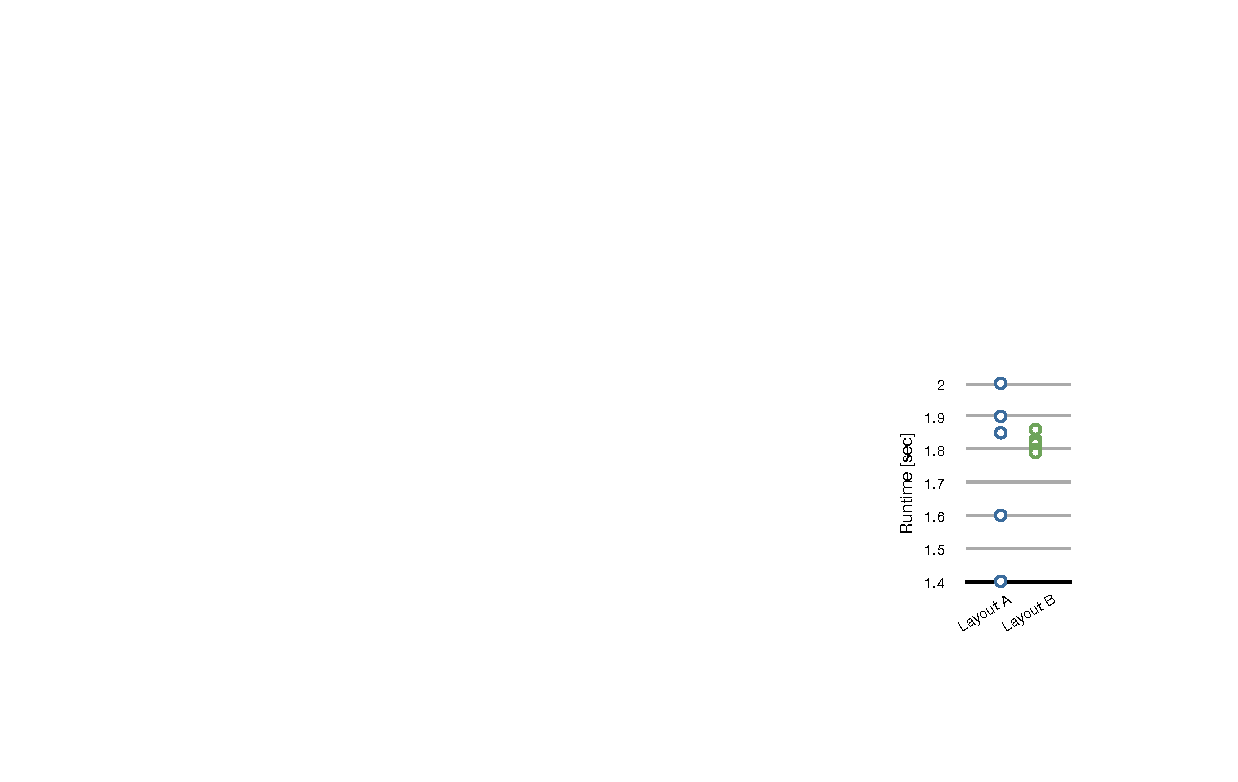
\includegraphics[width=.18\textwidth]{pdf/methodology_runtimes.pdf}
\vspace{-15pt}
\caption{Query times for two different layouts, each measured five times}  
\label{fig:methodology_runtimes}
\vspace{-10pt}
\end{wrapfigure}
However, if we take a look at the runtimes of all 5 runs in Figure~\ref{fig:methodology_runtimes}, we can see that Layout~A has a high variance (0.06), whereas the query time for Layout~B is rather stable (it's variance is 0.00075). Most system designers would probably prefer Layout~B, due to its performance being more predictable. This example demonstrates that reporting the average runtime alone is not sufficient for comparing two solutions~\cite{jain1991art}. Therefore at a minimum the variance or standard deviation of the sample should be provided along with the average to get a proper description of the sample.

We should keep in mind that when experimentally comparing multiple systems, we only get a \textit{sample} of their performance metrics which can only be used to \textit{estimate} the populations' performance metrics. Thus, there is always a level of uncertainty in our estimates, which renders the necessity of expressing this uncertainty in some way. One possible way to do this is to use confidence intervals, which express in natural language: ``There is a 95\% chance that the actual average runtime of System~A is between 1.7 and 1.8 seconds.''

\begin{table}[!b]
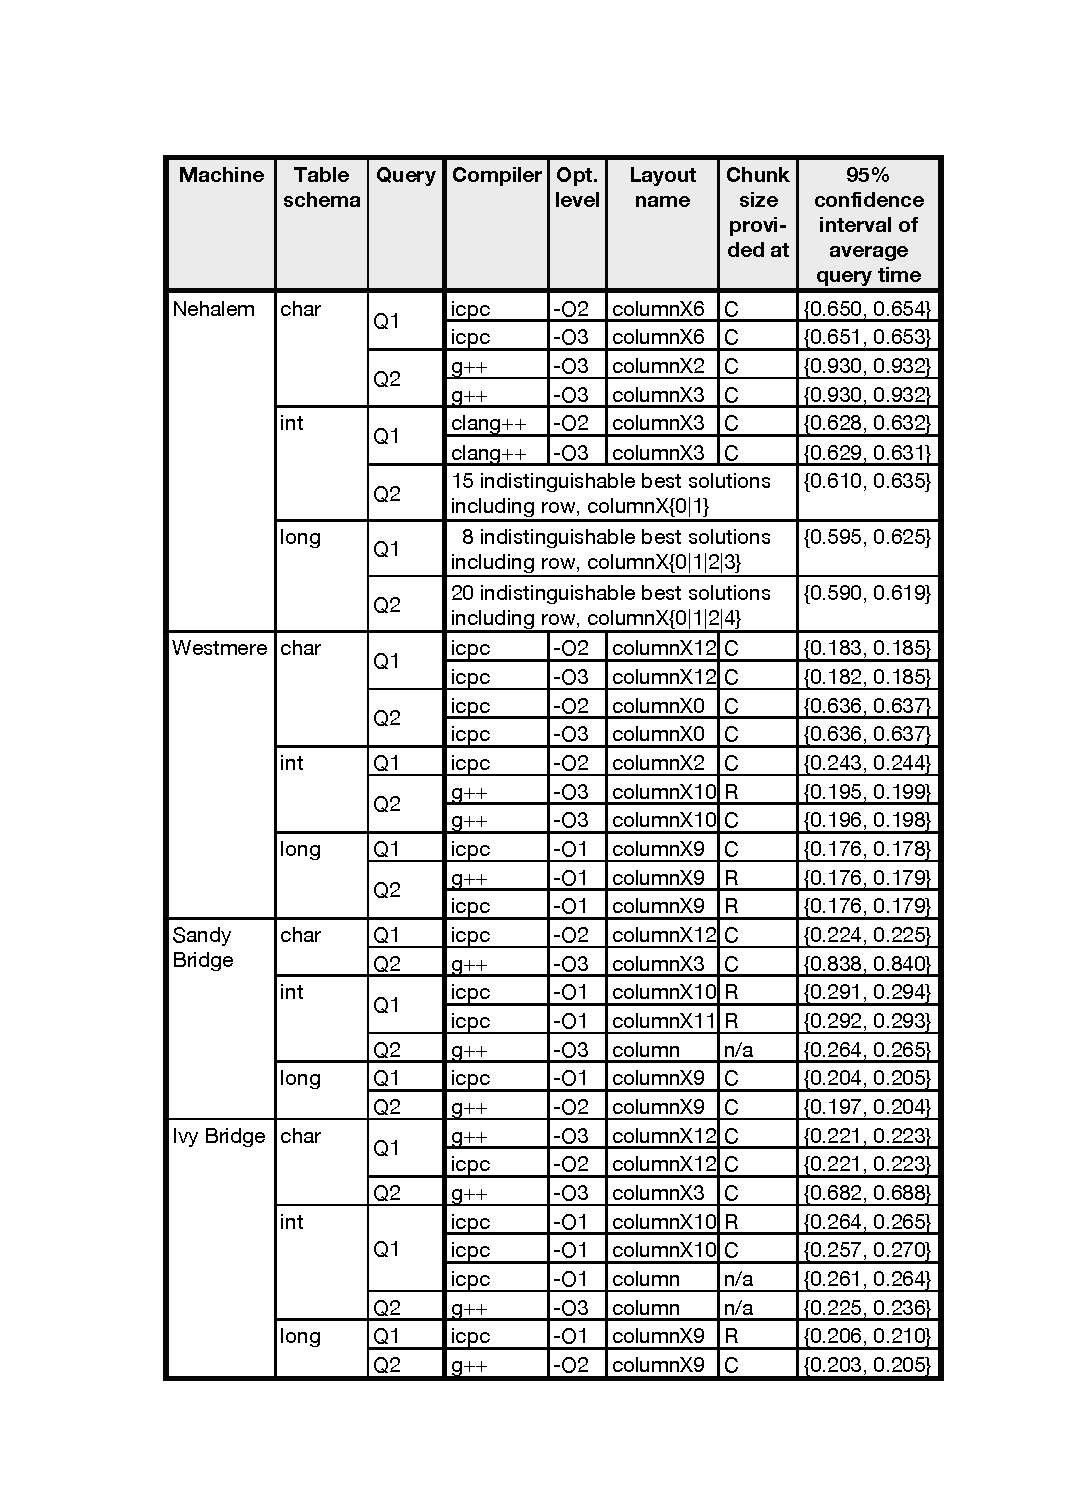
\includegraphics[width=.478\textwidth]{pdf/problem_bests_table.pdf}
\vspace*{-20pt}
\caption{The best layouts and most efficient ways of implementing a given query on a given table and executed on a given machine.}  
\label{fig:problem_bests_table}
%\vspace{-10pt}
\end{table}

\noindent\textbf{Confidence intervals.}
To create a confidence interval we first have to choose our confidence level, typically 90\%, 95\% or 99\%, denoted by $1 - \alpha$, where $\alpha$ is called the significance level. 
%A higher level of confidence yields a wider confidence interval for the same sample. The use-case determines the suitable confidence level, however, the latter trade-off has to be kept in mind when choosing one.
We require the sample size $n$, the sample mean $\overline{x} $, sample standard deviation $\sigma$, and the significance level $\alpha$. Then the confidence interval is defined as follows: $( \overline{x} - C \times \frac{\sigma}{\sqrt{n}} , \overline{x} + C \times \frac{\sigma}{\sqrt{n}}) $, where $C$ is the so-called confidence coefficient.
The choice of the confidence coefficient is determined by the sample size~\cite{jain1991art}. If we have a large sample ($n \geq 30$), we can use the $1 - \alpha / 2$-quantile of the standard normal distribution for the confidence coefficient: $C = Z_{1-\alpha / 2}$. However, we ran only 5 measurements, thus we have a sample size of $n=5$. Therefore, we should only use the $1 - \alpha / 2$-quantile of the Student's t-distribution with $n-1$ degrees of freedom: $C = t_{[1-\alpha / 2 , n-1]}$. The prerequisite is that the population needs to have a normal distribution, which is a fair assumption for our runtime measurements.
%To illustrate the difference between these two coefficients: for $\alpha = 0.05$, and $n = 5$ we get $Z_{0.975} = 1.96$ and $t_{[0.975, 4]} = 2.776$, thus for a small sample we get a wider confidence interval due to the confidence coefficient alone.
For instance, the 95\% confidence intervals for our example in Figure~\ref{fig:methodology_runtimes} are:  (0.23,~3.27) for Layout~A, and (1.65,~1.99) for Layout~B. This makes Layout~B a safer choice, if predictability is of great importance for the system designer. (See~\cite{jain1991art} for details.)
When looking at the measured query times on Layout~A in Figure~\ref{fig:methodology_runtimes}, we can see that the relatively wide confidence interval for Layout~A is due to the large variance of the sample: the points are scattered  out across the (1.4,~2.0) interval. However, a sample can have a large variance even if most measured values are ``near" to each other, and only a few of them having a higher or lower value than the rest. These latter are called outliers. 

\noindent\textbf{Outlier detection.}
An outlier is an element of a sample that does not ``fit" into the sample in some way. It is hard to quantify the criteria for labelling an element as an outlier, and it also depends heavily on the use-case. Therefore, the most common technique used for detecting outliers is plotting the sample on a scatter plot, and visually inspecting the plot by a human.
If we assume, that there is only one outlier in the sample, and it is either the minimum, or the maximum value, than we can use Grubb's test~\cite{grubbs1950sample} to automatically detect outliers. The only problem is that this method tends to identify outliers too often for samples with less than eight elements. This explains why it detected an outlier in 27\% of the cases in our experiments. To counter the error rate of the method we have included an additional condition for labelling an outlier: $\text{margin\_or\_error} / \overline{x} \geq$ 2.5\%, where the margin of error is defined as the radius of the confidence interval. This reduces the detection rate to 3\%, and those elements proved to be outliers after manual inspection.

\noindent\textbf{Choosing the best solution when there is no single best solution.}
Choosing the best solution using the average runtime is easy, we simply take the one with the smallest one. We have also seen that this can be arbitrarily wrong, and that is why confidence intervals provide a better basis of comparison than the sample mean. 
However, comparing confidence intervals is not that straight-forward as comparing scalars. If two intervals are disjoint, they are easily comparable. It they are not disjoint, and the mean of one sample is inside the other sample's confidence interval, they are indistinguishable from each other with the same level of confidence, as that of the intervals. Finally, if they are not disjoint, but their means do not fall into the other sample's interval, an independent two-sample t-test (Welch's t-test~\cite{welch1947generalization}) can decide whether they are distinguishable, and if so, which one is better.

\vspace*{-0.2cm}

\section{Results}


Table~\ref{fig:problem_bests_table} displays our recommendations for choosing a data layout and implementation strategy for each machine, schema and query\footnote{We have noticed that varying the chunk size of chunked column-layouts between $2^{12}$ and the biggest possible one ($2^{30}$ for Table\_char, $2^{28}$ for Table\_int, and $2^{27}$ for Table\_long) does not make a significant difference in the query times, regardless of the query, machine, and compiler. Thus, we have excluded those results from our discussion.
}. Notice that in some cases there are multiple best solutions. Looking at these results the question arises: what influences the choice of best solution? Thus, let us investigate the connection between the elements of the parameter space and the best layout. %For this we have calculated the relative occurrence of a layout as the best solution, aggregated over the values of each parameter (machine, schema, query, compiler, and O-level). Here we have taken special care to weight multiple best solutions of a problem with the reciprocal of their count.

\begin{figure}[!h]
\vspace{-5pt}
\centering
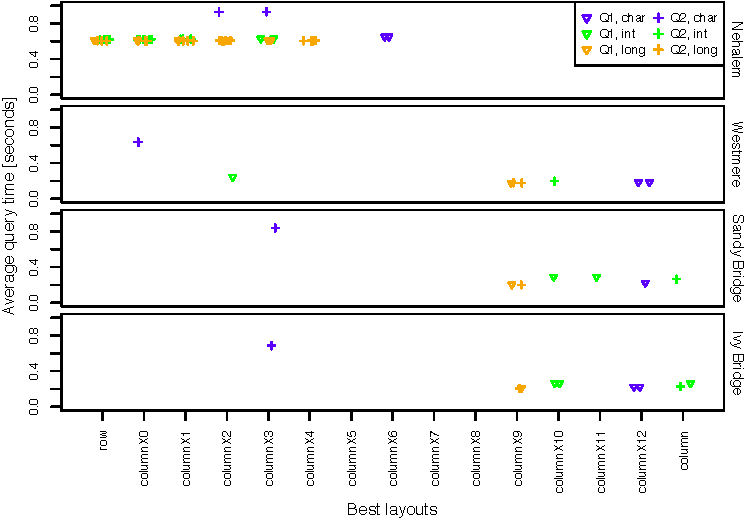
\includegraphics[width=0.48\textwidth]{pdf/problem_bests_plot.pdf}
\vspace{-20pt}
\caption{Best layouts and their query times. Drilled-down along machine, schema, and query.}  
\label{fig:problem_bests_plot}
\vspace{-10pt}
\end{figure}

\begin{figure*}[!ht]
\centering
\MultiplotChart[width=.97\textwidth, height=.641\textwidth, xunit={Relative size of the set of best solutions}, yunit={Slowdown compared to best solution}, xCount=6, yCount=4, yValues={["runtimeA AS [engine A]", "runtimeB AS [engine B]", "runtimeA AS [engine A]", "runtimeB AS [engine B]"]}, xValues={["date <= '2008/05/10'", "date > '2008/05/10'", "date <= '2008/05/10'", "date > '2008/05/10'", "date <= '2008/05/10'", "date > '2008/05/10'"]}, rightArr={["Nehalem", "Westmere", "Sandy Bridge", "Ivy Bridge"]}, topArr={["Q1, char", "Q2, char", "Q1, int", "Q2, int", "Q1, long", "Q2, long"]}, forceXequal, forceYequal, yFirst, options={"legend": { "show": true }, "axis": { "x": { "tick": { "fit":true } } }}]{SELECT date, ? FROM data2 WHERE ?;}
\caption{Robustness graphs for 24 different experiments displaying the impact of non--optimal layouts on runtime performance. The horizontal axis displays the k-th-best data layout picked (where $k$ is in 1$,\ldots, N=$252; normalized to 100\%). The vertical axis displays the performance overhead of that method over the best one (displayed till at most 250\% overhead; notice that some curves leave their plot).
The bigger the area under the curve, the more likely it is that a decision for a non-optimal data layout will trigger a performance loss. }  
\label{fig:fragility}
\vspace{-10pt}
\end{figure*}

In Figure~\ref{fig:problem_bests_plot} we can see the query times of the best layouts, drilled-down along machine, schema, and query. We can immediately notice the radical difference between Nehalem and the other three CPU architectures. The oldest one, Nehalem, prefers layouts with smaller chunk sizes, i.e.~close to row layout. The three newer ones on the other hand prefer larger chunk sizes, i.e.~close to column layout. For the latter CPUs we can further notice that the best layout for a dataset is often the one, where the following holds: \texttt{2~* field\_size * chunk\_size = 4KB} --- which is when the chunk perfectly fits the memory page: columnX12 for \texttt{char}, columnX10 for \texttt{int} and columnX9 for \texttt{long}.

\begin{table}[!ht]
  \vspace{-10pt}
  \scriptsize
  \centering
  \begin{tabular}{| l || r | r | r | r | r | r |}
    \hline
\multirow{2}{*}{\bf Machine}  &  \multicolumn{2}{c|}{\bf char} &  \multicolumn{2}{c|}{\bf int} & \multicolumn{2}{c|}{\bf long} \\ \cline{2-7}
 & {\bf Q1} & {\bf Q2} & {\bf Q1} & {\bf Q2} & {\bf Q1} & {\bf Q2} \\ \hline \hline
Nehalem & 11.2 & 6.6 & 2.7 & 2.6 & 2.0 & 2.0 \\ \hline
Westmere & 29.6 & 6.7 & 3.7 & 4.7 & 3.7 & 2.8 \\ \hline
Sandy Bridge & 20.6 & 5.2 & 4.3 & 4.5 & 2.9 & 2.8 \\ \hline
Ivy Bridge & 14.4 & 4.3 & 3.2 & 3.7 & 2.6 & 2.3 \\ \hline
    \end{tabular}
    \vspace{-5pt}
    \caption{The quotient of worst and best query times for each experiment. We observe up to a factor 29.6 difference in runtime.}
    \label{tab:fragility}
    \vspace{-5pt}
    \end{table}
So far we have seen the best solutions, but have not talked about the performance of the other ones. In Table~\ref{tab:fragility} we show the ratio of the worst and the best query times, drilled-down along machine, schema, and query. For \texttt{char} we can get factor 4 to factor 29 worse by choosing the wrong layout and/or compiler. At this point it would be interesting to know, how does the best solution's runtime compare to the others solutions' runtimes?

%When looking at the plots in Figure~\ref{fig:fragility} we can note that best solutions for \texttt{char} and Q1 excel in performance, as only 5\% of the solutions have a query time that is at most 50\% worse than the best.



% When looking at the results per machine in Figure~\ref{fig:table_layout_machine}, we can see that our oldest machine, with the Nehalem CPU, prefers layouts with smaller chunk sizes. However, the newer CPUs prefer layouts with larger chunk sizes. We get more insight into the latter phenomena when looking at the connection between the schema and the layout in Figure~\ref{fig:table_layout_schema_all}. Here we can notice that the best layout for a dataset is most often the one, where the following holds: size(field) * chunk\_size = 2KB. Finally, the query doesn't influence too much which layout is the best, as seen in Figure~\ref{fig:table_layout_query_all}.

% It is an interesting question, whether the compiler and O-level have an effect on the performance of the layouts, i.e.~which one is chosen as the best one. TODO: The relative occurrence of a layout as the best solution, aggregated over each compiler and O-level can be seen in Figure~\ref{fig:tables_solution_layout}. We can conclude that the compiler and O-level does not make too much of a difference of a given layout, yet this doesn't mean that all compilers are equally efficient. When looking at the Compiler column in Figure~\ref{fig:problem_bests} we can see that \texttt{icpc} (50\%) and \texttt{g++} (46\%) are the most efficient ones, and \texttt{clang++} (4\%) was rarely providing the best runtime.
\vspace*{-0.2cm}

\section{Robustness Graphs}

In Figure~\ref{fig:problem_bests_plot} we could already observe that the set of best layouts for a particular experiment is not always considerably faster than the second or even the $k$-th-best method. A~database architect may be willing to live with a data layout that is suboptimal for a very specific case, but does not incur too much performance overhead in the general case. To facilitate this decision, we introduce robustness graphs. Given runtime measurements for $N$ different methods ($N=252$ in our case), we depict the overhead of the $k$-th best method over the best method set. The result for 24 different experiments is shown in Figure~\ref{fig:fragility}. The robustness graphs show that for some situations, e.g.~Q1 on \texttt{char} run on Sandy Bridge, one should be more careful in choosing the layout than in others, e.g.~Q2 on \texttt{long} run on Westmere. We are planning to explore these kind of graphs as a general technique in a longer  paper.

\section{Conclusions and Guidelines}

Our guideline for choosing the best layout is as follows:
For servers equipped with a Nehalem CPU it is a safe bet to use row layout, while for machines with the subsequent Westmere, Sandy Bridge, and Ivy Bridge architectures it is just fine to use column layout. For the latter machines we can exploit the schema for some fine-tuning, by creating PAX--blocks with the same size as the virtual memory pages. Having branches in the query is an additional argument for this optimization. The compiler, O-level, and compile time vs. runtime layouts will not change the choice of best layout, but they are to be chosen carefully for the best performance.

We have shown how misleading it can be to choose the best solution along means. Take the case of Q1 on \texttt{long} run on Nehalem, where 20\% of all possible solutions are statistically indistinguishable from best solutions with 95\% confidence.

\noindent {\bf Acknowledgments.} Research supported by BMBF.

% ensure same length columns on last page (might need two sub-sequent latex runs)
\balance

\vspace{-5pt}

\scriptsize
\bibliographystyle{abbrv}
\bibliography{chunkedColumns}

\end{document}